\if 0\begin{figure*}[t]
    \centering
    \subfigure[Network scan: Throughput timeline.] {
        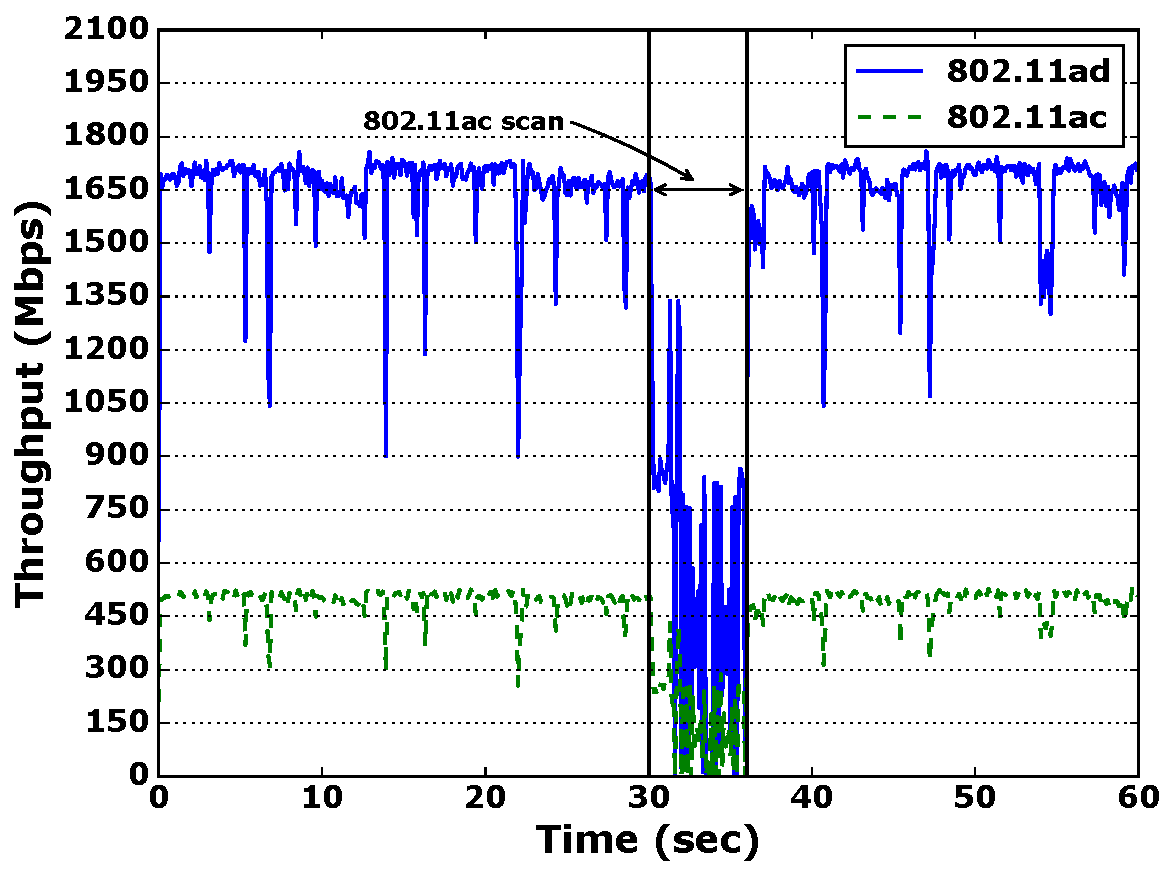
\includegraphics[scale=0.23]{NetworkManagerScan/timeline_no_fix.pdf}
        \label{fig:scan_issue}
    }\hfill
    \subfigure[802.11ac contention: Timeline showing throughput drop during contention.] {
        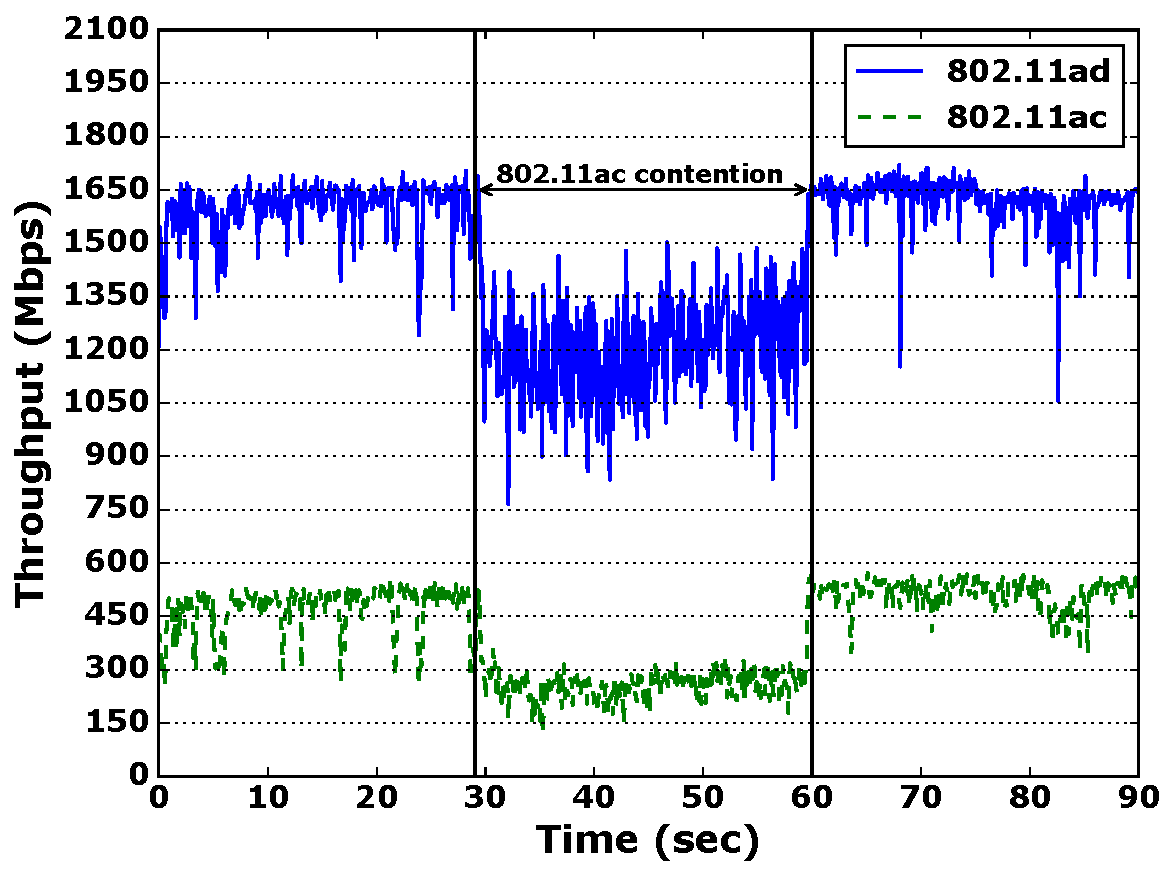
\includegraphics[scale=0.23]{contention/timeline.pdf}
        \label{fig:contention_timeline}
    }\hfill
    \subfigure[802.11ad blockage: 802.11ad throughput drop after re-connection.] {
        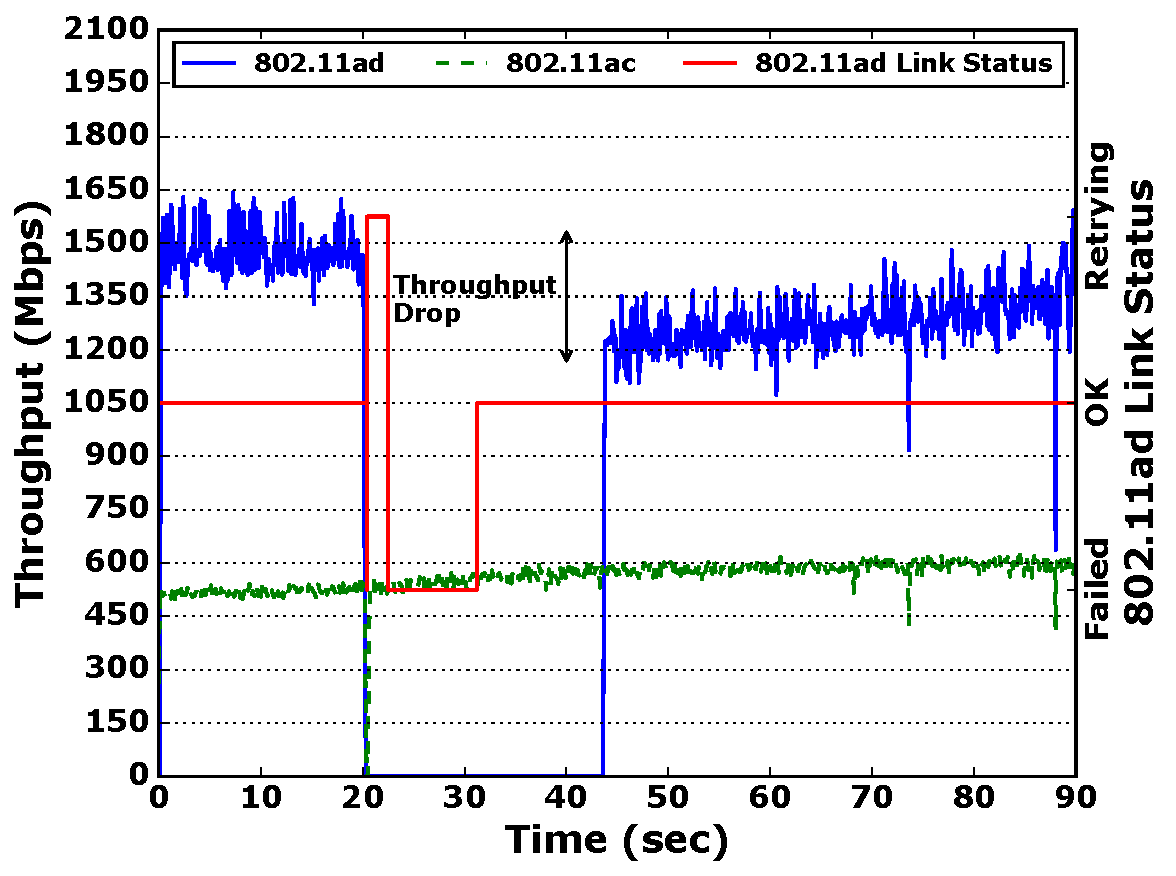
\includegraphics[scale=0.23]{blockage/blockage_tput_drop.pdf}
        \label{fig:blockage_tput_drop}
    }
    \vspace{-0.15in}
    \caption{Performance issues.}
    \vspace{-0.1in}
\end{figure*}
\fi
\begin{comment}
\begin{figure}[t]
    \centering
%    \subfigure[Network Scan (Timeline).] {
%        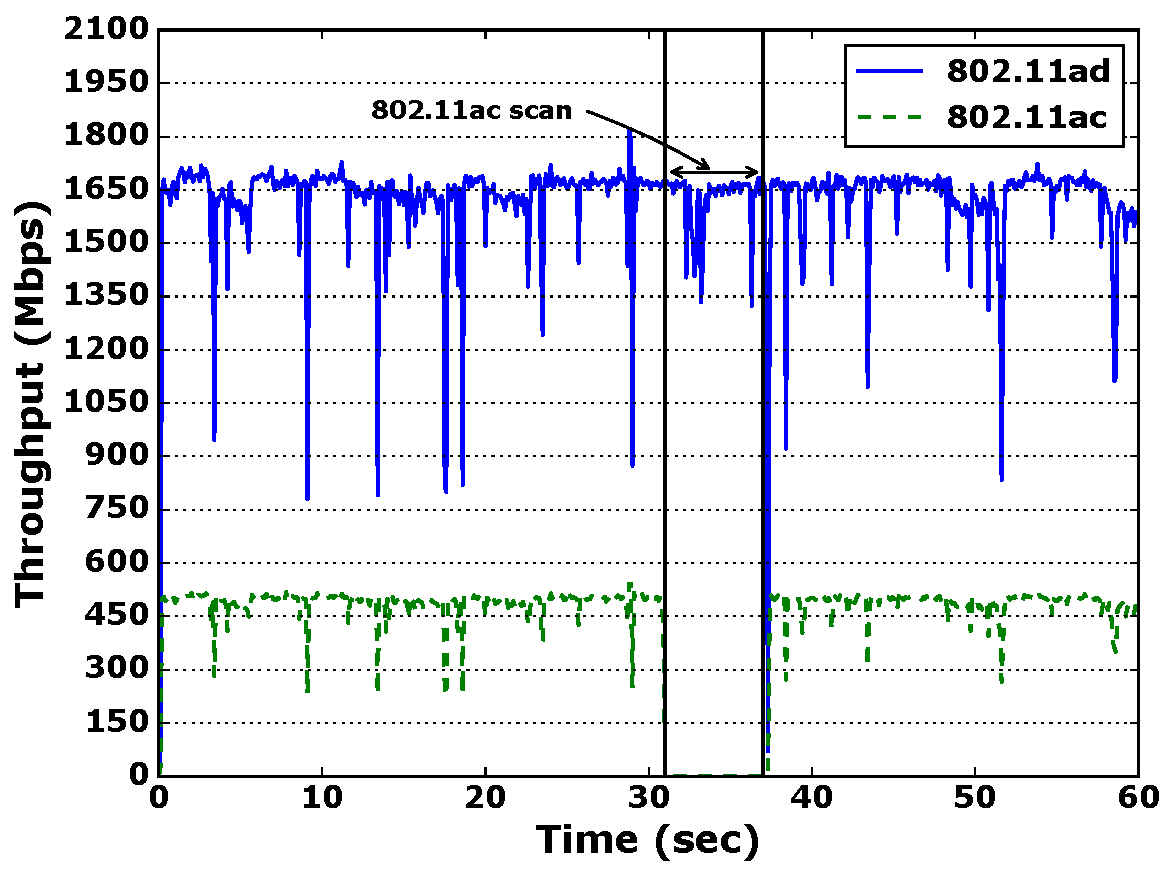
\includegraphics[scale=0.25]{NetworkManagerScan/timeline_fix.pdf}
%        \label{fig:scan_fixed}
%    }\hfill
    \subfigure[\emph{minRTT} vs. \emph{FixedRatio}.] {
        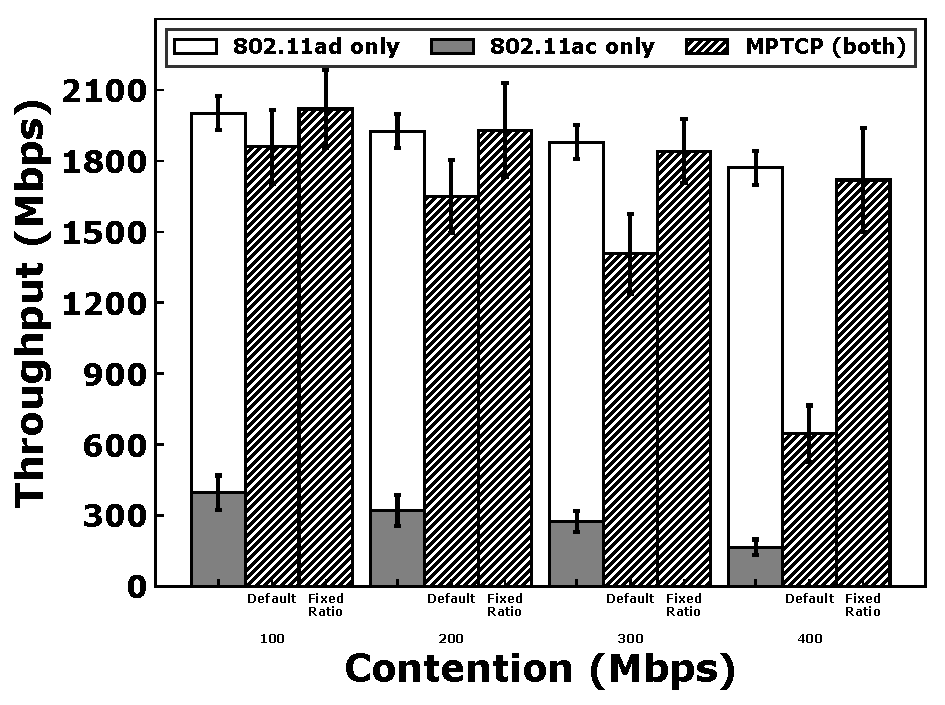
\includegraphics[scale=0.25]{contention/barplot.pdf}
        \label{fig:contention_barplot}
    }\hfill
    \subfigure[802.11ad Blockage: Improved recovery time.] {
        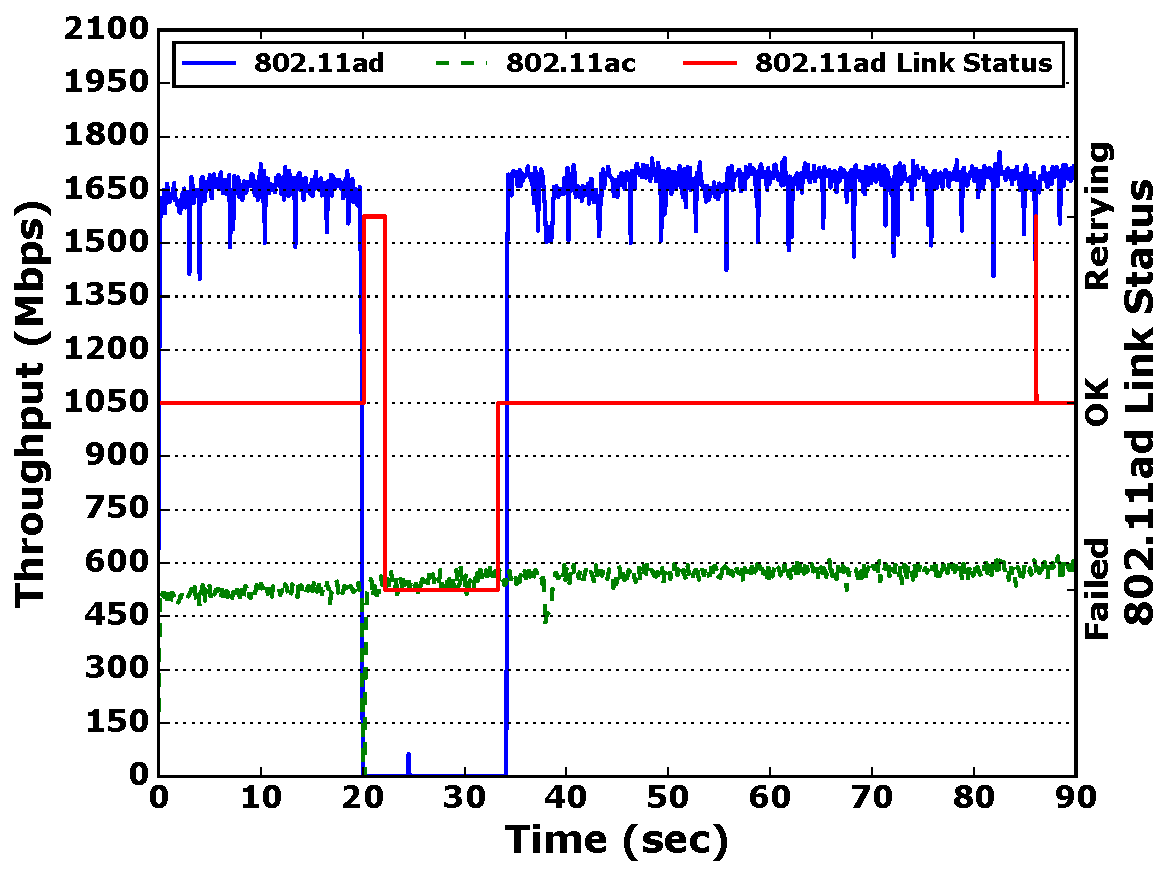
\includegraphics[scale=0.2]{blockage/blockage_fixed.pdf}
        \label{fig:blockage_recovery}
    }
    \vspace{-0.2in}
    \caption{\name evaluation.}
    \vspace{-0.2in}
\end{figure}
\end{comment}
Next, we turn our attention to dynamic environments involving network
scans, 802.11ac contention, or blockage of the 802.11ad link. We
observe that the default MPTCP architecture is unable to adapt,
yielding sub-optimal performance.
%are extremely challenging for
%the current MPTCP architecture
We then design and implement \name, a new
MPTCP scheduler that addresses the root-cause of this performance
degradation. \name consists of three parts:

\noindent\textbf{\name-SCAN}. During an 802.11ac scan, 802.11ad throughput also suffers severely, as the packet
scheduler, unaware of the scan, assigns packets in the same ratio as before the scan.
\name-SCAN
arbitrates the network scan requests generated
from the user space and disables the scheduling of packets to the
subflow where the request has been made for the duration of the
network scan, resulting in a 2.2x throughput improvement on average. 
%However, disabling future scheduling alone may not be
%enough to prevent packets from being held-up in the TCP queues or at
%any of the buffers in the lower layers of the network stack. We thus
\if 0
We
adopt a two-step approach, where \name: (1) stops the assignment of
packets to subflow about to undertake scanning and (2) waits for the
subflow-level \emph{send-queue} to be emptied out. We observe that
%Fig.~\ref{fig:scan_fixed} shows 
%a timeline consisting of 802.11ac scan (marked as "802.11ac scan") but 
with \name's network scan management solution applied 
%during the scan period. We can clearly see (compared
%to the scan period in Fig.~\ref{fig:scan_issue}) that 
the 802.11ad throughput remains unaffected during the scan interval. 
\fi
%We repeated the
%measurements several times and observed \textbf{2.2x} performance gain on average.
\\
\noindent\textbf{\name-CONTENTION}. During 802.11ac contention,
the 802.11ad subflow is also
affected negatively.
\name-CONTENTION leverages our findings regarding the 
existence of a unique MPTCP throughput-optimal ratio, for given
subflow throughputs. The reaction to contention is to set the
packet-assignment ratio to match the ratio of the throughputs of the
802.11ad and 802.11ac subflows, accounting for the drop in 802.11ac
throughput due to contention. This leads to significant throughput
gains which increase with the amount of cross-traffic.
%We test our solution under different
%amounts of contention (from 100 Mbps to 400
%Mbps). Fig.~\ref{fig:contention_barplot} shows the expected sum, after
%accounting for 802.11ac throughput reduction in the presence of
%contention, and MPTCP performance under the default
%and \emph{FixedRatio} scheduler, which uses the optimal ratio for a
%given amount of contention. In all cases, \emph{FixedRatio}'s
%throughput is close to the expected sum while the default scheduler's
%throughput can be much lower.
\\
\noindent\textbf{\name-BLOCKAGE}. Although the 802.11ad link is restored 
%at the $31^{st}$ second, 
almost immediately after blockage is removed, 
MPTCP does not resume traffic on the 802.11ad subflow for
%another $\sim$12 seconds until the $43^{rd}$ second. 
10s of seconds.
\if 0
We found that 
%in
%the case of a timeout-based loss event, 
TCP congestion-control 
%sets
marks
%the {\tt pf} flag on the socket, indicating 
the flow to be
\emph{potentially failed}. The MPTCP scheduler 
%treats subflows with
%the {\tt pf} flag set as being unavailable and 
does not schedule any
packets on it. TCP congestion-control, on the other hand, is waiting
for an ACK to 
%unset the {\tt pf} flag 
unmark the flow as \emph{potentially failed} and 
%enter the {\tt
%  TCP\_CA\_RECOVERY} state that can restore the \emph{cwnd} to the
%value before the loss event, 
recover the \emph{cwnd} value but no packets are being directed to
the 802.11ad subflow.
% only a subflow-level re-transmission of the
%802.11ad subflow can trigger the transmission of an ACK on the
%receiver side.
%However, multiple timeout-based losses during the
%blockage period can lead to excessively high retransmission timeouts,
%and consequently to long delays before an ACK is received.
\fi
Additionally, on
resumption, the 802.11ad subflow often starts with a \emph{cwnd} and
\emph{ssthresh} that are half of their pre-loss
values, yielding suboptimal throughput. 
%Fig. \ref{fig:blockage_tput_drop} shows a sample timeline
%where the 802.11ad flow resumes to 1350 Mbps instead of 1650
%Mbps. 
%This results in a return to suboptimal throughputs.
%Note that this behavior depends on the exact specifics of the
%TCP congestion-control state at the time it enters the recovery
%state. 
%Nonetheless, we observed this quite often and it does have a
%non-negligible impact on throughput.
\name-BLOCKAGE reduces the delay in resuming traffic over the 802.11ad
subflow to less than 1 s
by resetting the {{\tt pf}} flag to allow for traffic to be
scheduled on the 802.11ad subflow and uses the TCP's window recovery
mechanism to restore the \emph{cwnd} (and consequently throughput) to the value just before loss the
event. 
%However, we found that this alone
%was not enough to resume the traffic flow on the 802.11ad
%interface. 
\if 0
Also, 
when the 802.11ad link is blocked, the
subflow-level \emph{cwnd} is cut to 1, with packets in flight also
equal to one. As a result, the scheduler is unable to schedule any new
packets on 802.11ad subflow since the \emph{cwnd} is reported as being
full. In order to overcome this, \name uses the TCP's window recovery
mechanism to restore the \emph{cwnd} to the value just before loss the
event. 
\fi 
%In contrast to Fig.~\ref{fig:blockage_tput_drop}, where MPTCP resumed traffic on the
%802.11ad subflow after a 12 s delay,
%With \name engaged 
%(Fig. \ref{fig:blockage_recovery}) 
%MPTCP starts using the 802.11ad interface in less than 1s after link re-establishment. This
%is a vast reduction in delay for resuming traffic on the subflow.
In a dynamic environment, where such blockage events will occur quite
frequently, \name's gains would translate into a significant
improvement in user-experience.
